\chapter{Theory and motivation}
\label{sec:Theory}

\section{The Standard Model of Particle Physics}
The Standard Model of particle physics (SM) is a relativistic and renormalisable quantum field theory, that combines the electroweak theory developed by Glashow, Salam and Weinberg \cite{SM_Glashow, SM_Salam, SM_Weinberg} with quantum chromodynamics (QCD), the theory of the strong interactions.
It combines the current knowledge of fundamental particles and their interactions at microscopic level with the exception of gravitation.

The electroweak theory is already a combination of the electromagnetic and the weak interaction.
Every fundamental particle can interact via the weak force.
For instance, the weak force is responsible for the $\beta$-decay of neutrons.
Atoms or molecules are bound by the electromagnetic interaction taking place between electrically charged particles.
If particles also carry a so-called colour charge, they can interact via the strong interaction, which binds e.g. protons and neutrons in a nucleus.

In the Standard Model, matter arises as half-integer spin particles from quantum fields.
These particles are called \textsc{Fermions} and can be furthermore split up in \textsc{Quarks} and \textsc{Leptons}.
There exist 6 so-called ``flavours" of quarks: up (\uquark), down (\cquark), charm (\cquark), strange (\squark), top (\tquark) and bottom\footnote{The bottom quark is sometimes also called beauty.} (\bquark).
According to their mass and other physical properties, they can be grouped into three generations:
\begin{align*}
    \begin{pmatrix} \uquark \\ \dquark \end{pmatrix},
    \begin{pmatrix} \cquark \\ \squark \end{pmatrix},
    \begin{pmatrix} \tquark \\ \bquark \end{pmatrix}.
\end{align*}
Quarks in the top row are referred to as \textsc{Uptype} quark.
They carry an electrical charge of $+\frac{2}{3}e$, whereas \textsc{Downtype} quarks carry a charge of $-\frac{1}{3}e$.
Thus, they can participate in the electromagnetic interaction.
In addtion, quarks carry colour charge allowing them to interact via the strong interactions.

Leptons do not carry flavour as opposed to quarks.
There exist three flavours of leptons, namely the electron (\en), the muon (\mun) and the tauon (\taum) with an electric charge of $-e$ and their neutral counterparts, the neutrinos \neue, \neum, \neut.
Similarly to quarks, the leptons can be grouped into three generations
\begin{align*}
    \begin{pmatrix} \en \\ \neue \end{pmatrix},
    \begin{pmatrix} \mun \\ \neum \end{pmatrix},
    \begin{pmatrix} \taum \\ \neut \end{pmatrix}.
\end{align*}
As the neutrinos do neither carry electrical nor colour charge, they only interact weakly.
Due to that fact it is not possible to detect neutrinos at hadron colliders like the \lhc.
For each fermion, there exists a corresponding antifermion with same mass, but opposite quantum numbers.

In the Standard Model, the interactions among the particles are described by the mediation of spin-1 gauge bosons.
For the electromagnetic interaction, this is the electric neutral photon \g.
It couples to electrically charged particles.
Since the photon is massless the range of the electromagnetic interaction is infinite.
The weak interaction is mediated by three massive gauge boson.
The electrically charged \Wp and \Wm as well as the neutral \Z boson.
The \Wpm bosons only couple to left-handed fermions (or right-handed antifermions), whereas the \Z couples to both, left- and right-handed fermions, but with different strength.
Due to their large mass of $m_{\Wpm} \approx 80 \gev$ and $m_\Z \approx 91 \gev$ the weak interaction is only short-ranged.
The strong interaction is carried by 8 massless gluons.
They couple to particles carrying a colour charge and carry colour itself.
Thus, there is also a gluon-gluon coupling possible leading to a QCD coupling strength \as, which strongly depends on the momentum transfer in an interaction.
For low energies \as increases dramatically, which means that coloured particles cannot be isolated.
This phenomenon is called \textsc{Confinement}.
At high energies \as is very small resulting in the \textsc{Asymptotic Freedom}, i.e. the quarks are thus quasi-free while keeping short distances.
Due to the confinement, \textsc{Hadrons}, strongly interacting composite particle, must always be colour-neutral.
They exist either as quark-antiquark system and are called \textsc{Mesons} or as composite of three quarks and are named \textsc{Baryons}.
Recent \lhcb measurements report the observation of candidates for bound states consisting of 4 quarks (2 quark, 2 antiquarks) \cite{Tetraquark} and also 5 quarks (4 quarks, 1 antiquark) \cite{Pentaquark}.

Contradicting to the properties of the particles mentioned above, the invariance of local gauge transformation requires that the particles of the Standard Model are massless.
This problem is solved by the \textsc{Higgs mechanism}, which introduces a doublet of complex scalar (spin 0) fields.
The potential of thies field spontaneously breaks the electroweak symmetry and leads to massive bosons and fermions due to interaction with the Higgs field.
The Higgs mechanism furthermore predicts a massive spin-0 particle, the \textsc{Higgs Boson}.
As lastly unobserved particle, its discovery in July 2012 by \atlas \cite{Higgs_ATLAS} and \cms \cite{Higgs_CMS} was a big success for the experimental community as well as for the theory of the Standard Model itself. 
Figure \ref{fig:SM} summarises the fermions and bosons of the Standard Model and list their main properties \cite{Perkins_HEP, Burgess_SM, Meissner}.
\begin{figure}[ptb]
    \centering
	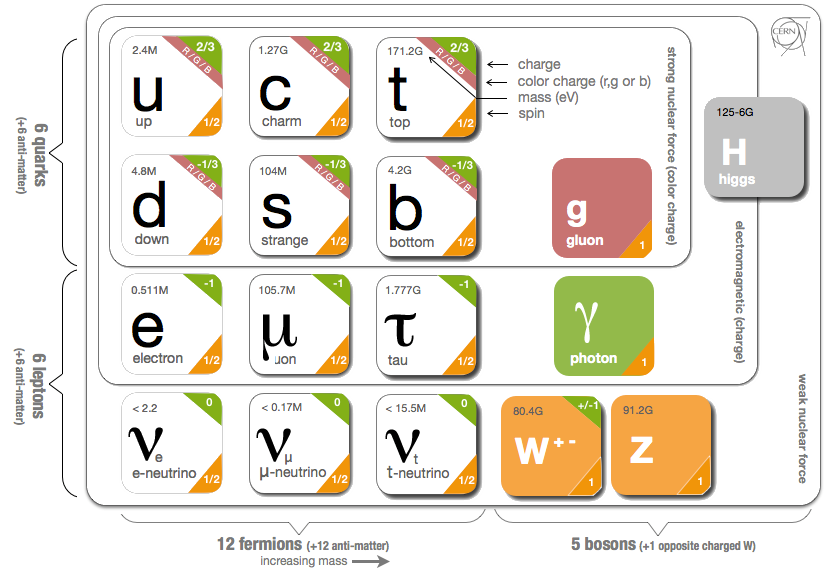
\includegraphics[width=\textwidth]{Standard_Model}	
	\caption{Summary of all fundamental fermions and bosons of the Standard Model of particle physics with their most important properties. Figure slightly modified and taken from \cite{SM_figure}.}
	\label{fig:SM}
\end{figure}

\section{Baryons}

\section{Resonances}

\section{Methods of parameter estimation}
This section briefly describes two methods to estimate parameters, which are used in this thesis.

\subsection{Maximum-Likelihood method}
A common task in High Energy Physics is to find the best estimate for a set of parameters $\vec{\theta}$ by a measurement of some variables $\vec{x}$.
As an example one wants to measure the mass $m_X$  and the width $\Gamma_X$ of a particle $X$ decaying into two daughter particles $A$ and $B$, i.e. $X \to AB$.
For this purpose one would measure the energies $E$ and momenta of $p$ multiple times.
Thus the set of measured variables would be $\vec{x} = (E_A, \vec{p}_A, E_B, \vec{p}_B)$ and one would try to find the ``best" value for the parameters $\vec{\theta} = (m_X, \Gamma_X)$. 
The most frequently used method for the estimate of $\vec{\theta}$ is the \textsc{Maximum-Likelihood Method}.
Given a theoretical prediction of the measured distribution in form of a probability density function $f(\vec{x}|\vec{\theta})$ one can define the likelihood function
\begin{align}
    \mathcal{L}(\vec{x}|\vec{\theta}) := \prod_{i=1}^{N} f(\vec{x}_i|\vec{\theta}),
\end{align}
where $N$ denotes the number of (independent) measurements.
The maximum of this likelihood function $\mathcal{L}$ with respect to $\vec{\theta}$ is assumed to be the best estimate of $\vec{\theta}$.
Practically one minimises equivalently $-\log(\mathcal{L})$ for computational reasons.

Often, a probability density function $P$ is a linear combination of several components, e.g. a signal and background component $P_\text{sig}$ respectively $P_\text{bkg}$.
Thus the number of events $N$ is a random variable as well.
If $N$ obeys the Poisson distribution the so-called \textsc{Extended Likelihood Function} can be defined as: 
\begin{align}
    &\mathcal{L}_\text{ext}(\vec{x} | \Nsig, \Nbkg, \vec{\theta}) :=  \nonumber \\ 
    &\qquad \frac{(\Nsig+\Nbkg)^N\exp{(\Nsig+\Nbkg)}}{N!} \prod_{i=1}^{N} \left[f_\text{sig}P_\text{bkg}(\vec{x}_i|\vec{\theta}) + f_\text{bkg}P_\text{bkg}(\vec{x}_i|\vec{\theta})\right],
\end{align} 
where $N_j$ denotes the corresponding yield and $f_j:=\frac{N_j}{N}$ the fraction of signal respectively background component.
Thus the maximisation of the extended likelihood function $\mathcal{L}_\text{ext}$ enables to estimate the yields of each component at the same time \cite{Lista_Statistics, PDG}.

\subsection{Beeston-Barlow method}
\label{sec:BeestonBarlow}
When one tries to estimate the composition of a data sample it might happen that there does not exist an analytic form of the distribution.
Thus, one relies on simulations and has to bin the data into $n$ bins.
This gives a set of numbers ${d_i}$ with $i \in [1,n]$, where $d_i$ denotes the number of data events in falling into bin $i$.
Let $j$ denote a source contained in the data, $P_j$ its strength and $a_{ji}$ the number of simulated events from source $j$ in bin $i$, then the predicted number of events in bin $i$ is given by
\begin{align}
    f_i := N_\text{D} \sum_{j=1}^{m} \frac{P_j a_{ji}}{N_j},
\end{align}
where $N_\text{D}$ is the total number of events in the data sample, $N_j$ the number of simulated events for source $j$ and $m$ the number of sources.
Starting from a Poisson distributed probability of observing a particular $d_i$ as
\begin{align}
    \mathrm{e}^{f_i} \frac{f_i^{d_i}}{d_i!}
\end{align}
the logarithmic likelihood to be maximised looks like
\begin{align}
    \log \mathcal{L} = \sum_{i=1}^{n} \left[d_i \log(f_i) - f_i\right] \label{eq:BinnedLL}
\end{align}
after dropping the constant factorials.
This likelihood function is also known as \textsc{Binned Likelihood}.

Nonetheless, the binned likelihood of equation (\ref{eq:BinnedLL}) does not account for finite sizes of the simulation samples.
Due to large computation times simulation samples are often small and there are non-negligible statistical fluctuations in the $a_{ji}$.
Thus the likelihood function has to be modified as follows:
The predicted number of events in a bin is now
\begin{align}
    f_i := N_\text{D} \sum_{j=1}^{m} \frac{P_j A_{ji}}{N_j},
\end{align}
where $A_{ji}$ is the unknown expected number of events for source $j$ in bin $i$.
The ``observed" $a_{ji}$ in the simulation sample is generated from $A_{ji}$ by a Poisson distribution\footnote{Actually, the $a_{ji}$ obey a binomial distribution. However, for $A_{ji} << N_j$ it can be approximated by a Poisson distribution.}.
Thus, the probabilities of observing a set of ${d_i}$ and ${a_ji}$ have to be combined and the likelihood function to be maximised is
\begin{align}
    \log \mathcal{L} = \sum_{i=1}^{n} \left[d_i \log(f_i) - f_i\right] + \sum_{i=1}^{n} \sum_{j=1}^{m} \left[a_{ji} \log(A_{ji}) - A_{ji}\right]. \label{eq:BBLL}
\end{align}
Throughout this analysis, the maximisation of this likelihood function in equation (\ref{eq:BBLL}) is referred to as \textsc{Beeston-Barlow Method} \cite{BeestonBarlow}.
